\documentclass[a4paper,11pt]{article}

\usepackage[english]{babel}
\usepackage[utf8]{inputenc}
\usepackage{amsmath}
\usepackage{amssymb}
\usepackage{mathtools}
\usepackage{graphicx}
\usepackage[colorinlistoftodos]{todonotes}
\usepackage[lmargin=1.in,rmargin=1.in,tmargin=1.in,bmargin=1in]{geometry}
\usepackage{authblk}
\usepackage{setspace}
\usepackage{natbib}

\newcommand{\Prob}{\mathrm{P}}

\usepackage{xcolor}
\usepackage{adjustbox}
\usepackage{verbatim}
\definecolor{shadecolor}{rgb}{.9, .9, .9}
\newenvironment{code}%
   {\par\noindent\adjustbox{margin=1ex,bgcolor=shadecolor,margin=0ex \medskipamount}\bgroup\minipage\linewidth\verbatim}%
   {\endverbatim\endminipage\egroup}

\newenvironment{codeSmall}%
   {\par\noindent\adjustbox{margin=1ex,bgcolor=shadecolor,margin=0ex \medskipamount}\bgroup\minipage\linewidth\verbatim\footnotesize}%
   {\endverbatim\endminipage\egroup}
   

\title{The Gambler's Ruin Problem}
\author{Brian Weinstein - bmw2148}
\affil{Probability \& Statistics (STAT-W4700), Columbia University, Fall 2015}
\date{December 15, 2015}

\begin{document}
\maketitle
%\doublespacing

\nocite{*}



\section{Problem Statement}

In the Gambler's Ruin Problem, we have a gambler $A$ and a casino $B$, who are playing a game against each other. The total combined fortune of the two is $k$ dollars, with the gambler starting with $i$ dollars, and the casino starting with $k-i$ dollars, where $i$ and $k-i$ are known positive integers. On each play of the game, the probability that $A$ will win one dollar from $B$ is a known value $p\in\left(0,1\right]$, and the probability that $B$ will win one dollar from $A$ is $1-p$.

Suppose that the game is played repeatedly (and independently) until the fortune of either $A$ or $B$ is reduced to 0 dollars.



\section{Problem Solution}
Let $a_i$ denote the probability that gambler $A$ will reach $k$ dollars before they reach 0 dollars, given that their initial fortune is $i$ dollars. Since each play of the game is independent of the others, we can think of the problem essentially start over on each play, with the only difference being that the ``initial'' fortunes of the gambler and casino have changed. The value of interest is $a_i$ for $i\in\{0,1,\ldots,k-1,k\}$.

\subsection{Solution for $i \in \{0,k\}$}
\label{sec:solntrivial}

The cases of $i=0$ and $i=k$ are trivial. When $A$ runs out of money they can no longer play, and thus $a_0=0$, and when $A$ wins all $k$ dollars, the casino can no longer play, and thus $a_k=1$. Finding $a_i$ when $i\not\in\{0,k\}$ is nontrivial and is solved in Section \ref{sec:solnnontrivial} below.

\subsection{Solution for $i \in \{1,2,\ldots,k-2,k-1\}$}
\label{sec:solnnontrivial}

Define the following events:
\begin{itemize}
\item $A_1$ is the event in which the gambler wins one dollar (i.e., the casino loses one dollar) on the first play of the game,
\item $B_1$ is the event in which the casino wins one dollar (i.e., the gambler loses one dollar) on the first play of the game, and
\item $W$ is the event in which the gambler wins all $k$ dollars before reaching $0$ dollars.
\end{itemize}

By the Law of Total Probability, we see that
\begin{align}
\Prob(W)&=\Prob(A_1)\Prob(W|A_1)+\Prob(B_1)\Prob(W|B_1) \nonumber 
\\
&=p\Prob(W|A_1)+(1-p)\Prob(W|B_1).
\label{eqn:lawoftotalprob}
\end{align}

Since the gambler starts with $i$ dollars, we see that $\Prob(W)=a_i$, as defined earlier. If the gambler wins on the first play, they'd now have $i+1$ dollars, and by our assumption that each game play is independent, we see that $\Prob(W|A_1)=a_{i+1}$. Similarly, if the gambler loses on the first play they'd now have $i-1$ dollars, and therefore $\Prob(W|B_1)=a_{i-1}$.

By Equation \ref{eqn:lawoftotalprob}, we find
\begin{equation}
a_i=p a_{i+1} + (1-p) a_{i-1}.
\label{eqn:defai}
\end{equation}

By plugging in $i=1,2,\ldots,k-2,k-1$ into Equation \ref{eqn:defai}, we get $k-1$ equations
\begin{align}
a_1 &= p a_2 + (1-p) a_0 = p a_2 \nonumber
\\
a_2 &= p a_3 + (1-p) a_1 \nonumber
\\
& \vdotswithin{=} \nonumber
\\
a_{k-2} &= p a_{k-1} + (1-p) a_{k-3} \nonumber
\\
a_{k-1} &= p a_{k} + (1-p) a_{k-2} = p + (1-p) a_{k-2},
\label{eqn:exampleai}
\end{align}
where we can simplify our equations for $a_1$ and $a_k-1$ by using $a_0=0$ and $a_k=1$, as defined in Section \ref{sec:solntrivial}.

We can rewrite these $k-1$ equations as
\begin{align}
a_2 - a_1 &= \frac{1-p}{p} (a_1 - a_0) = \left(\frac{1-p}{p}\right) a_1 \nonumber
\\
a_3 - a_2 &= \frac{1-p}{p} (a_2 - a_1) = \left(\frac{1-p}{p}\right)^2 a_1 \nonumber
\\
a_4 - a_3 &= \frac{1-p}{p} (a_3 - a_2) = \left(\frac{1-p}{p}\right)^3 a_1 \nonumber
\\
& \vdotswithin{=} \nonumber
\\
a_{k-1} - a_{k-2} &= \frac{1-p}{p} (a_{k-2} - a_{k-3}) = \left(\frac{1-p}{p}\right)^{k-2} a_1 \nonumber
\\
a_{k} - a_{k-1} = 1 - a_{k-1} &= \frac{1-p}{p} (a_{k-1} - a_{k-2}) = \left(\frac{1-p}{p}\right)^{k-1} a_1
\label{eqn:exampleairewritten}
\end{align}
and by equating the sum of the left sides of these equations with the sum of the right sides of these equations, we find
\begin{equation}
1-a_1 = a_1 \sum_{i=1}^{k-1} \left( \frac{1-p}{p} \right)^i .
\label{eqn:airelation}
\end{equation}

\subsubsection{Solution When $p=0.5$}
\label{sec:solnfiargame}

When $p=0.5$ (i.e., when the game is fair), we use Equation \ref{eqn:airelation} to solve for $a_1$,
\begin{equation}
1-a_1 = a_1 \sum_{i=1}^{k-1} \left( \frac{1-0.5}{0.5} \right)^i = a_1 \sum_{i=1}^{k-1} \left( 1 \right)^i = a_1 \left(k-1\right) \ \ \ \ \Rightarrow \ \ \ \ a_1 = \frac{1}{k}.
\end{equation}
We can then use the recurrence relation in Equation \ref{eqn:exampleairewritten} to recursively solve for $a_2, \ldots, a_{k-1}$, from which we find
\begin{equation}
a_i = \frac{i}{k} \ \ \mathrm{for} \ \ i \in \{ 1, 2, \ldots, k-2, k-1 \}.
\end{equation}




\subsubsection{Solution When $p\neq0.5$}
When $p\neq0.5$ (i.e., when the odds of the game are skewed in favor of either the gambler or the casino), we can rewrite Equation \ref{eqn:airelation} as
\begin{equation}
1-a_1 = a_1 \frac{ \left(\frac{1-p}{p}\right)^k - \left(\frac{1-p}{p}\right) }{ \left(\frac{1-p}{p}\right) - 1 },
\end{equation}

and then solving for $a_1$ we find
\begin{equation}
a_1 = \frac{ \left(\frac{1-p}{p}\right) - 1 }{ \left(\frac{1-p}{p}\right)^k - 1 }.
\end{equation}

In an identical method to that used in Section \ref{sec:solnfiargame}, we use the recurrence relation in Equation \ref{eqn:exampleairewritten} to recursively solve for $a_2, \ldots, a_{k-1}$, from which we find
\begin{equation}
a_i = \frac{ \left(\frac{1-p}{p}\right)^i - 1 }{ \left(\frac{1-p}{p}\right)^k - 1 } \ \ \mathrm{for} \ \ i \in \{ 1, 2, \ldots, k-2, k-1 \}.
\end{equation}

\section{Solution Summary}

Given the probability $p\in\left(0,1\right]$ that the gambler will win each play of the game, and given the initial fortune $i$ of the gambler and the initial fortune $k-i$ of the casino, we can calculate the probability that each of them would the the first to run out of money.

The probability $a_i$ that gambler will reach $k$ dollars before they reach 0 dollars, given that they start with $i$ dollars is given by
\begin{equation}
a_i =
\begin{cases}
\frac{i}{k} & p=0.5\\
\frac{ \left(\frac{1-p}{p}\right)^i - 1 }{ \left(\frac{1-p}{p}\right)^k - 1 } & p\neq0.5
\end{cases} \ \ \ \ \mathrm{for} \ \ i \in \{ 0, 1, \ldots, k-1, k \}.
\end{equation}

For select values of $k$, plots of $a_i$ as a function of $i$ and $p$ are shown in Figure \ref{fig:ai_vs_i_p}.
\begin{figure}
\centering
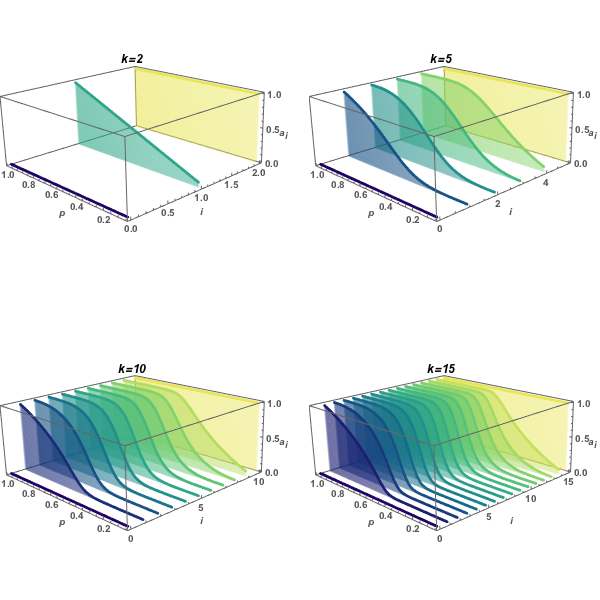
\includegraphics[width=1\textwidth]{plots.png}
\caption{\label{fig:ai_vs_i_p}Plots of $a_i$ as a function of $i$ and $p$, for select values of $k$. The Mathematica code used to generate the plots is shown in Appendix \ref{sec:mmcode}.}
\end{figure}

\pagebreak
\appendix
\section{Mathematica Code for Figure \ref{fig:ai_vs_i_p}}
\label{sec:mmcode}
\begin{codeSmall}
ai[i_, k_, p_] := Piecewise[{
   {i/k, p == 0.5},
   {(((1 - p)/p)^i - 1)/(((1 - p)/p)^k - 1), p != 0.5}}]

makePlot[k_] :=
 ListPointPlot3D[Flatten[
   Table[{i, p, ai[i, k, p]},
    {i, 0, k, 1},
    {p, 0.06, 0.99, 0.0045}], 1],
  AxesLabel -> {i, p, Subscript[a, i]}, 
  LabelStyle -> Directive[Darker[Gray], Bold, 10],
  ImageSize -> 300,
  ColorFunction -> 
   Function[{x, y, z}, ColorData["BlueGreenYellow"][x]],
  Filling -> Bottom, FillingStyle -> Directive[Thick, Opacity[0.2]],
  ViewPoint -> {-2.17, -2.37, 1.04}, 
  ViewVertical -> {-0.19, -0.24, 2.37},
  PlotLabel -> Style["k=" <> ToString[k], 12, Italic, Black]
  ]

GraphicsGrid[{{makePlot[2], makePlot[5]}, {makePlot[10], 
   makePlot[15]}}, ImageSize -> 600]
\end{codeSmall}

\bibliographystyle{plain}
\bibliography{gamblers-ruin-problem.bib}

\end{document}